\clearpage
\section{风中的草地}
在 Forge 中打开 \path{assets/scenes/Wind-Meadow.redflag}。层级里的“草地”是一个实体，选中后可以在“植被”组件里关闭风、改变株数或修改风向。“模型绘制”提供一丛草的网格和材质。植被配置保存这片地的分布种子、长宽和风的变化速度。调节时可直接看画面，按“保存植被配置”才把新数值写回所选的 YAML 文件。

\begin{center}
\panelimage{.76\linewidth}{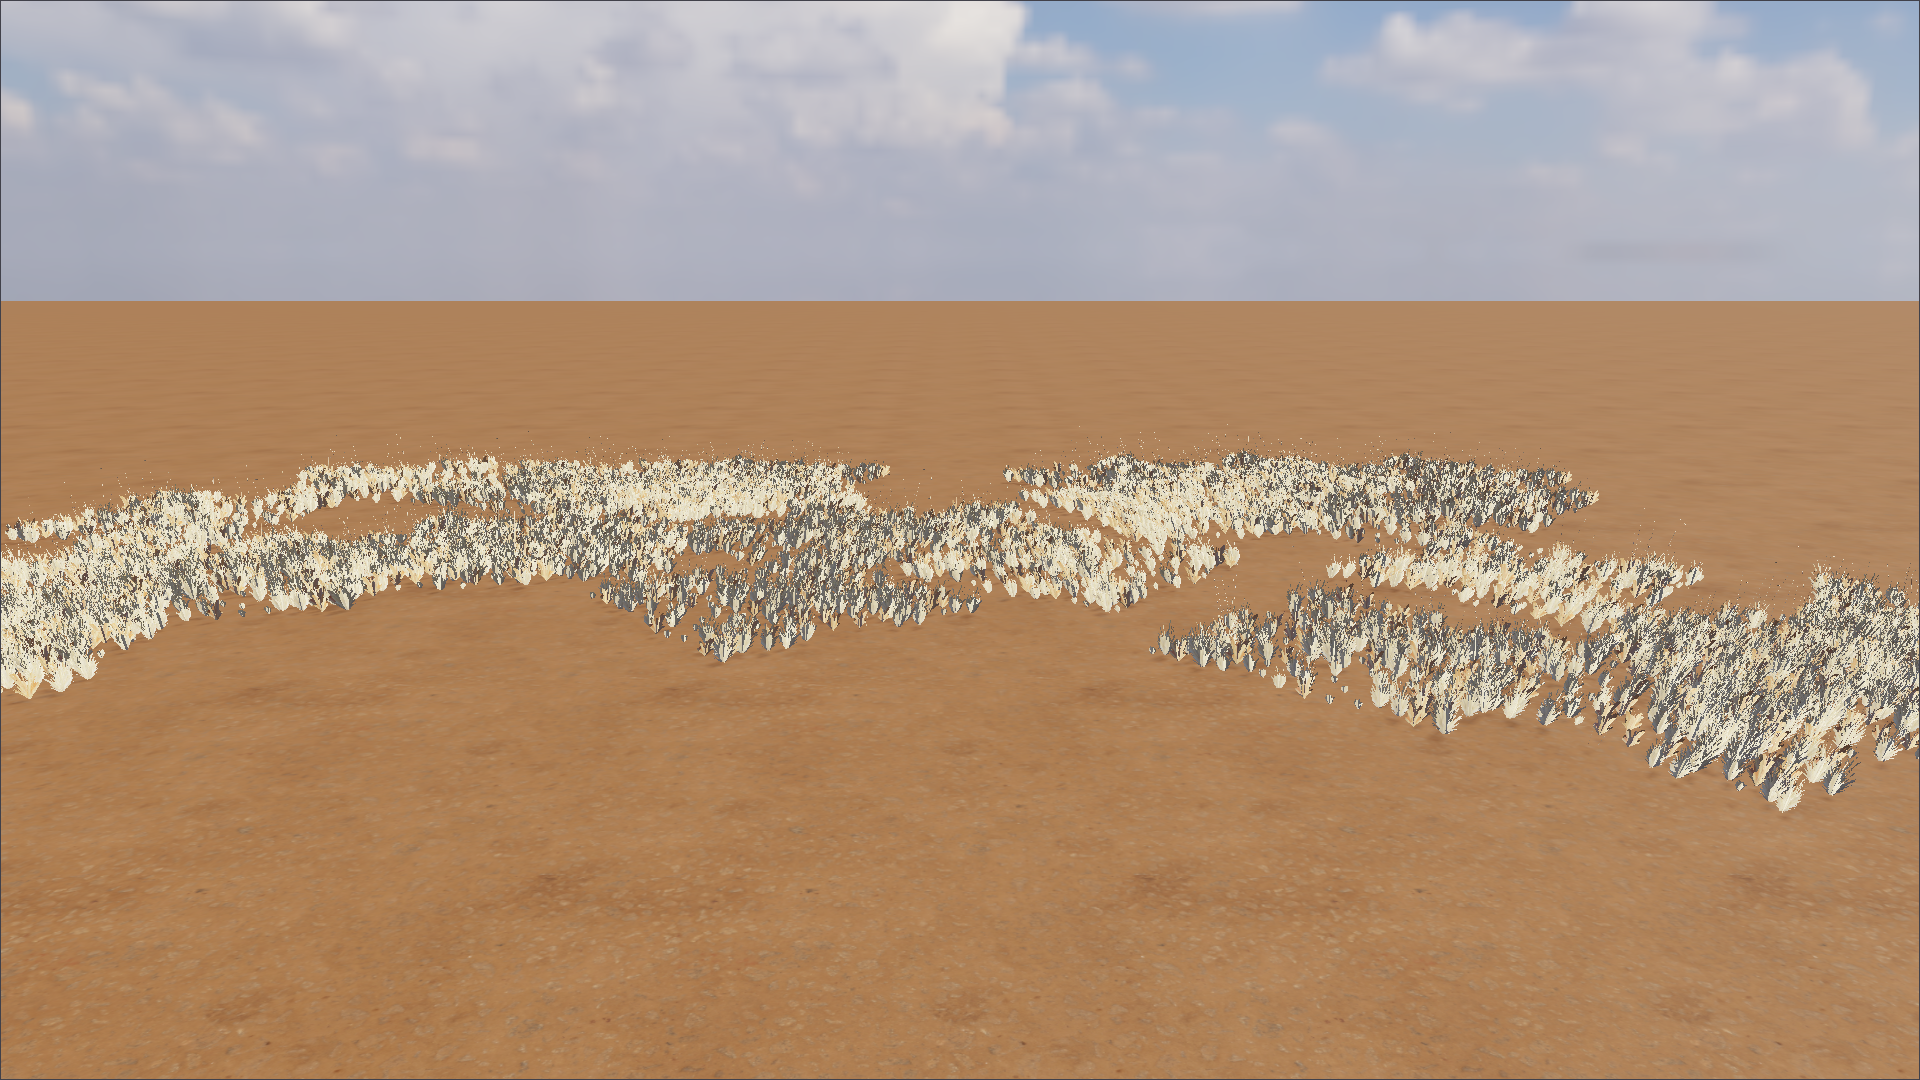
\includegraphics[width=\linewidth]{../../../output/validation/foliage/game.png}}{正式 Vulkan 游戏窗口，$1920\times1080$。草地使用 tevy 的 CC0 资源 Savanna Grass Patch。}
\end{center}

示例在 $12\times7$ 米内摆放 36 丛草。每丛的朝向和位置由同一个种子 17 决定，因此关风时不会换一批位置。模型缩小到原来的 0.42 倍，一丛高约 0.47 米。设 $h$ 为某个顶点离草根的高度，单位为缩放后的米，$\boldsymbol{x}$ 为这丛草在地块平面的位置，$\boldsymbol d$ 为单位风向。顶点的水平位移为
\[
 \Delta\boldsymbol{x}=h\,a\sin\!\left(2\pi
       \bigl(f t-\boldsymbol d\cdot\boldsymbol x/\lambda\bigr)\right)\boldsymbol d .
\]
顶点在草根时 $h=0$，整阵风吹过来也不会移动它。示例中 $a=0.28$，意味着每一米高度最多偏斜 0.28 米。$f=0.55$ 次/秒，$\lambda=6$ 米。从一丛草顺着风走 6 米，同一时刻两丛草摇到相同的位置。数值由这片小草地选定，增大 $a$ 会让叶尖移动得更远，减小 $\lambda$ 会让相邻草丛更容易朝不同方向倾斜。

\path{Redflag/src/Redflag/Renderer/Foliage.cpp} 的 \code{Place} 依据上式生成每丛草的矩阵。颜色、阴影和拾取共用本帧的矩阵。Vulkan 把矩阵排成连续的数组，再在 \code{vkCmdDrawIndexed} 中指定实例数。每换一丛草，显卡取下一个矩阵，顶点和贴图仍读同一份。这里按株倾斜，风沿单片叶子的弯曲以及草丛对间接光的逐帧遮挡尚未建模。
\readings{\refitem{https://developer.nvidia.com/gpugems/gpugems/part-i-natural-effects/chapter-7-rendering-countless-blades-waving-grass}{Kurt Pelzer，GPU Gems 第 7.4 节}\quad
\refitem{https://docs.vulkan.org/refpages/latest/refpages/source/vkCmdDrawIndexed.html}{Khronos，实例数量与索引绘制}\quad
\refitem{https://tevy.dev/models/savanna-grass-patch}{草地模型作者与资产}}
\clearpage

\subsection{同一片草地的两种画法}
对照程序把时间固定在 0.45 秒，先让 36 丛草分别绘制，再让一次绘制读取 36 份矩阵。两次都画一块砂石地面。回放中草地每丛有 4,464 个索引，实例化后的事件 21 一次画完 36 丛。场景内 60,884 个像素读到草地的实体编号，两种画法在全图 $960\times540$ 个位置读回的编号完全一致。

\begin{center}
\panelimage{.48\linewidth}{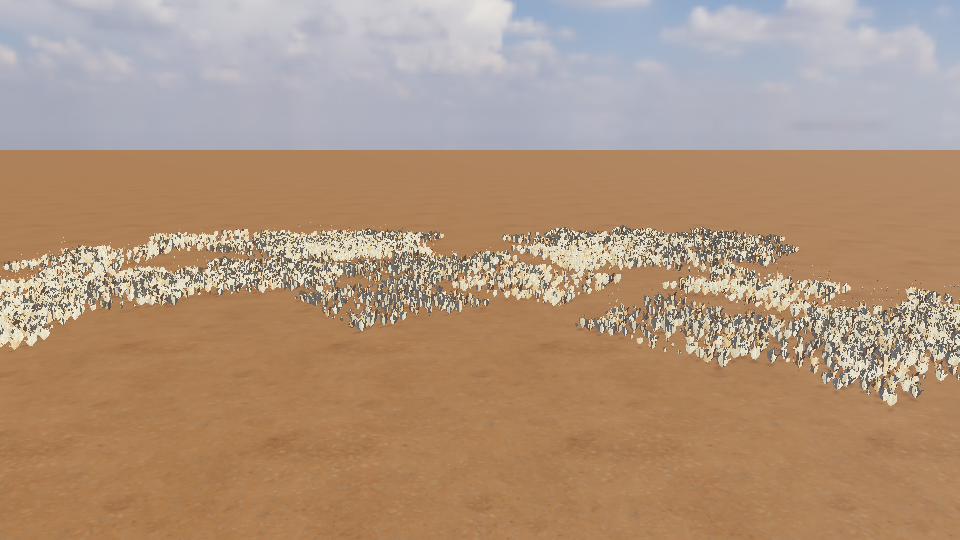
\includegraphics[width=\linewidth,trim=230 95 350 180,clip]{../../../output/validation/foliage/calm.png}}{取相同区域，关闭风}
\hfill
\panelimage{.48\linewidth}{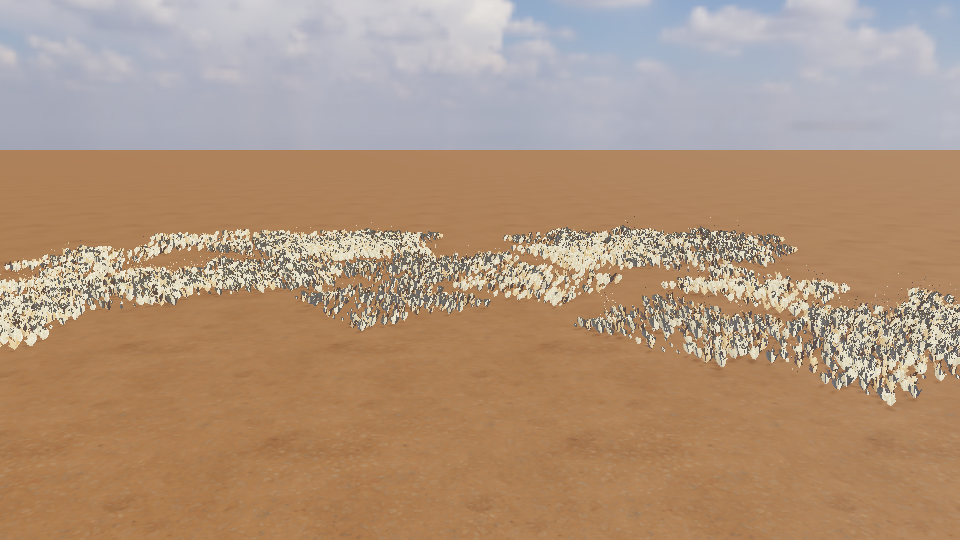
\includegraphics[width=\linewidth,trim=230 95 350 180,clip]{../../../output/validation/foliage/wind-045.png}}{开启风，0.45 秒}
\end{center}
\noindent 两张图取自实际 Forge 光照绘制。镜头、天空、太阳和曝光固定，关闭 TAA。放大看叶尖相对后排叶片的位置。两帧的整图有 71,863 个 RGBA 像素不同，包含移动的叶片与投影。另在草根不位于模型原点的数值例中检查了每丛的根部，最大位移为 0 米。

{\smalltable\noindent\begin{tabularx}{\linewidth}{@{}Xrrr@{}}\toprule
同一草地与地面 & 全场绘制次数 & CPU 录制（微秒） & GPU 绘制（微秒） \\\midrule
逐丛提交 & 37 & 235.10 & 30.912\\
实例化提交 & 2 & 127.95 & 31.312\\\bottomrule
\end{tabularx}}

在 RTX 5070 Ti Laptop GPU 上用 Debug/x64 测量。CPU 计时从开始记录场景到最后一个绘制命令写完，不含交换链等待或提交队列。两种方式按实例、逐丛、逐丛、实例轮换，每组先预热一帧再测 20 帧。表中是每种方式 40 帧的中位数。RenderDoc 1.47 分别回放两份真实帧，相同轮换顺序，每组先预热一次再采六次。GPU 一栏是颜色与实体编号阶段各个绘制事件耗时之和的中位数。单独计算草地得到 23.328 和 24.272 微秒。这个规模省下的是 CPU 命令开销。更大地块的逐块剔除、远景模型简化和叶片过密时的像素开销需要另测。

\readings{原图、全部 CPU/GPU 样本、复现命令见 \path{output/validation/foliage/}。测试入口为
\path{tests/FoliageTests.cpp}，回放脚本为 \path{tests/replay_foliage.py}。}
